
%%%%%%%%%%%%%%%%%%%%%%%%%%%%%%%%%%%%%%%%%%%%%%%%%%%%%%%%%%%%%%%%%%%%%%%%%%%%%%%%%%%%%%%%%%%%%%%%
% Hydrodynamik                                   
%%%%%%%%%%%%%%%%%%%%%%%%%%%%%%%%%%%%%%%%%%%%%%%%%%%%%%%%%%%%%%%%%%%%%%%%%%%%%%%%%%%%%%%%%%%%%%%%
\newpage
\subsection{Hydrodynamik}
	\subsubsection{Definitionen der Hydrodynamik}
		\begin{minipage}{19cm}
			\begin{itemize}
				\item \textbf{Abgeschlossene Fluidmenge:} ein Volumen, in welches keine Materie hinein oder heraus fliesst
				\item \textbf{Fluidteilchen:} ein materielles Fluidvolumen von sehr kleiner Ausdehnung
				\item \textbf{Geschwindigkeitsfeld:} ordnet jedem Punkt in einem Volumen eine Geschwindigkeit zu
				\item \textbf{Stationäre Strömung:} Geschwindigkeit, Druck, Dichte etc. ist zeitunabhängig
				\item \textbf{Stromlinie:} Kurven im Geschwindigkeitsfeld einer Strömung, deren Tangentenrichtung mit den Richtungen der Geschwindigkeitsvektoren übereinstimmen
				\item \textbf{Bahnlinie:} Eigentliche Bahn eines einzelnen Teilchens in einem Strömungsfeld
				\item \textbf{Laminare Strömung:} Strömung, in welcher die einzelnen Fluidteilchen sich in geordneten, nebeneinander gleitenden Schichten bewegen
				\item \textbf{Turbulente Strömung:} Strömung, in welcher Wirbel auftreten, wessen Kräfte entgegen der Bewegungsrichtung des Fluids wirken
			\end{itemize}
		\end{minipage}
	
	\subsubsection{Ideale Strömungen}
		\begin{minipage}{12cm}
			\myparagraph{Kontinuitätsgleichung (ideale Flüssigkeiten)}
				\begin{flushleft}
					Für eine inkompressible stationäre Strömung:
				\end{flushleft}
				\quad
				\renewcommand{\arraystretch}{2}
				\begin{tabular}{ p{5.5cm} | p{7cm}}
					$\Delta m_1 = \Delta m_2$	&	$m$ = Masse in $kg$\\
					$\underbrace{\rho \cdot A_1 \cdot v_1 \cdot \Delta t}_{\Delta m_1} = \underbrace{\rho \cdot A_2 \cdot v_2 \cdot \Delta t}_{\Delta m_2}$	&	$\rho$ = Dichte Fluid in $\frac{kg}{m^3}$\\
					$A_1 \cdot v_1 = A_2 \cdot v_2$	&	$A$ = Querschnittsfläche Rohr in $m^2$\\
					$A \cdot v = \dot{V} = \dfrac{\Delta V}{\Delta t} = konstant$	&	$v$ = Flussgeschwindigkeit Fluid in $\frac{m}{s}$\\
					&	$\dot{V}$ = Volumenstrom in $\frac{m^3}{s}$\\
				\end{tabular}
				\renewcommand{\arraystretch}{1}
		\end{minipage}
		\begin{minipage}{10cm}
			\vspace{-\ht\strutbox}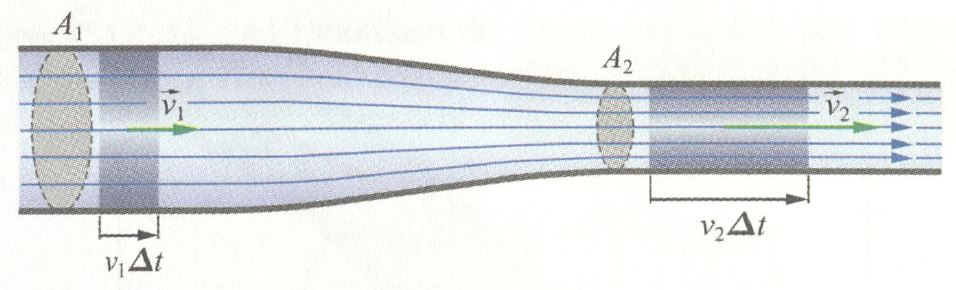
\includegraphics[width=7cm]{./bilder/Kontinuitaetsgleichung.jpg}
		\end{minipage}
		\newline
		\newline
		\newline
		\newline
		\begin{minipage}{12.5cm}
			\myparagraph{Bernoulli-Gleichung}
				\renewcommand{\arraystretch}{2.5}
				\begin{tabular}{ p{7.3cm} | p{4.5cm}}
					$\Delta W = \Delta W_{pot} + \Delta W_{kin}$	&	$\rho$ = Dichte Fluid in $\frac{kg}{m^3}$\\
					$W_{pot} = \underbrace{\rho \cdot A_2 \cdot \Delta s_2}_{\Delta m_2} \cdot g \cdot h_2 - \underbrace{\rho \cdot A_1 \cdot \Delta s_1}_{\Delta m_1} \cdot g \cdot h_1$	&	$A$ = Querschnittsfläche Rohr in $m^2$\\
					$W_{kin} = \underbrace{\rho \cdot A_2 \cdot \Delta s_2}_{\Delta m_2} \cdot \frac{1}{2} {v_2}^2 - \underbrace{\rho \cdot A_1 \cdot \Delta s_1}_{\Delta m_1} \cdot \frac{1}{2} {v_1}^2$	&	$s$ = von Fluid zurückgelegte Strecke in $m$\\
					$p_1 + \rho \cdot g \cdot h_1 + \rho \frac{{v_1}^2}{2} = p_2 + \rho \cdot g \cdot h_2 + \rho \frac{{v_2}^2}{2}$	&	$h_1$ = tiefer gelegener Rohrabschnitt in $m$\\
					$p + \rho \cdot g \cdot h + \rho \frac{{v}^2}{2} = konstant$	&	$h_2$ = höher gelegener Rohrabschnitt in $m$\\
				\end{tabular}
				\renewcommand{\arraystretch}{1.5}
				\begin{tabular}{ p{7.3cm} | p{7cm} }
					& $v$ = Flussgeschwindigkeit Fluid in $\frac{m}{s}$\\
				\end{tabular} 
				\renewcommand{\arraystretch}{1}
		\end{minipage}
		\begin{minipage}{10cm}
			\vspace{-\ht\strutbox}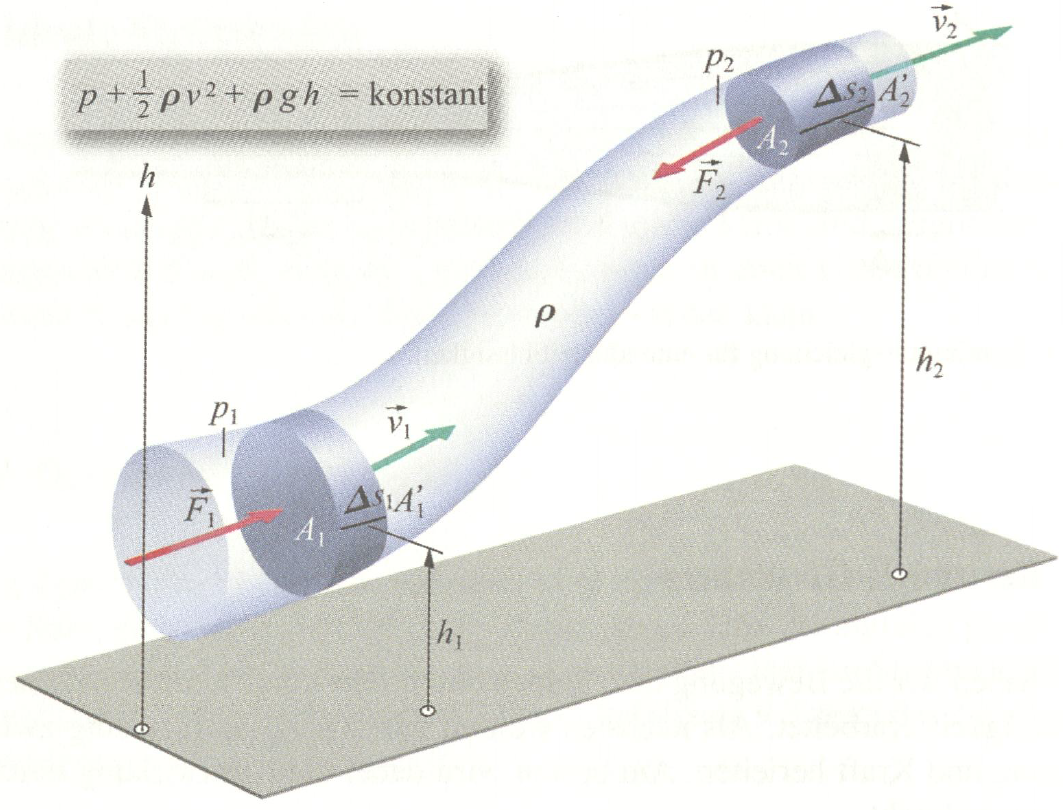
\includegraphics[width=7cm]{./bilder/BernoulliGleichung.png}
		\end{minipage}
		\newline
		\newline
		
		\myparagraph{Wirbelsatz von Thomson}
			\begin{minipage}{19cm}
				Die Zirkulation längs einer geschlossenen, materiellen Kurve in einem reibungsfreien, barotropen Fluid, auf das nur konservative Massenkräfte wirken, bleibt zeitlich konstant.
			\end{minipage}
		\newline
		\myparagraph{Wirbelsätze von Helmholtz}
			\begin{minipage}{19cm}
				\begin{enumerate}
					\item Die Zirkulation einer Wirbelröhre ist längs dieser Röhre konstant.
					\item Eine Wirbelröhre besteht immer aus denselben Fluidteilchen (wandert also mit).
					\item Die Zirkulation einer Wirbelröhre bleibt zeitlich konstant.
				\end{enumerate}
			\end{minipage}
		
		\subsubsection{Reale Strömungen}
			\begin{minipage}{12cm}
				\myparagraph{Newtonsches Reibungsgesetz}
				\begin{flushleft}
					Schubspannung: Spannung, welche eine an einem Körper parallel angreifende Kraft F verursacht.
				\end{flushleft}
				\renewcommand{\arraystretch}{2.5}
				\begin{tabular}{ p{4cm} | p{7cm}}
					$\tau = \dfrac{F_\parallel}{A} = \eta \dfrac{\mathrm{d}v}{\mathrm{d}z}$	&	$\tau$ = Schubspannung in $\frac{N \cdot s}{m^2} \cdot \frac{m}{s \cdot m} = \frac{N}{m^2}$\\
					$F_R = \eta \cdot A \dfrac{\mathrm{d}v}{\mathrm{d}z} = \tau \cdot A$ & $v$ = Geschwindigkeit Platte in $\frac{m}{s}$\\
				\end{tabular}
				\renewcommand{\arraystretch}{1.5}
				\begin{tabular}{ p{4cm} | p{10cm} }
					& $z$ = Dicke Fluidschicht in $m$\\
					& $A$ = parallel angreifende Fläche in $m^2$\\
					& $F_{\parallel} = F_R$ = parallel angreifende Reibungskraft in $N$\\
					& $\eta$ = dynamische Viskosität (Zähigkeit) in $\frac{kg}{ms} = \frac{N \cdot s}{m^2} = Pa \cdot s$\\
				\end{tabular} 
				\renewcommand{\arraystretch}{1}
			\end{minipage}
			\begin{minipage}{10cm}
				\vspace{-\ht\strutbox}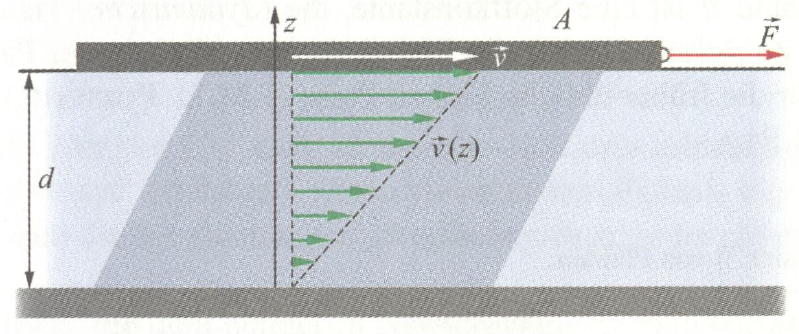
\includegraphics[width=7cm]{./bilder/NewtonschesReibungsgesetz.png}
			\end{minipage}
			\newline
			\newline
			\newline
			\newline
			\begin{minipage}{12cm}
				\myparagraph{Dynamische Viskosität (Zähigkeit), Fluidität}
				\renewcommand{\arraystretch}{2.5}
				\begin{tabular}{ p{4cm} | p{7cm}}
					$\eta = \tau \dfrac{\mathrm{d}z}{\mathrm{d}v}$	&	$\tau$ = Schubspannung in $\frac{N \cdot s}{m^2} \cdot \frac{m}{s \cdot m} = \frac{N}{m^2}$\\
					$\varphi = \frac{1}{\eta} = \dfrac{\mathrm{d}v}{\tau \cdot \mathrm{d}z}$	& $v$ = Geschwindigkeit in $\frac{m}{s}$\\
				\end{tabular}
				\renewcommand{\arraystretch}{1.5}
				\begin{tabular}{ p{4cm} | p{10cm} }
					& $z$ = Dicke Fluidschicht in $m$\\
					& $\eta$ = dynamische Viskosität (Zähigkeit) in $\frac{kg}{m \cdot s} = \frac{N \cdot s}{m^2} = Pa \cdot s$\\
					& $\varphi$ = Fluidität in $\frac{s^2}{kg \cdot m} \cdot m^2 \cdot \frac{m}{m \cdot s} = \frac{m \cdot s}{kg} = \frac{m^2}{N \cdot s} = \frac{1}{Pa \cdot s}$\\
				\end{tabular} 
				\renewcommand{\arraystretch}{1}
			\end{minipage}
			\newline
			\newline
			\newline
			\begin{minipage}[t]{16cm}
				\myparagraph{Reynoldszahl}
				\begin{flushleft}
					Einheitslose Zahl, welche den Übergang von einer laminaren in eine turbulente Strömung angibt.
				\end{flushleft}
				\renewcommand{\arraystretch}{2.5}
				\begin{tabular}{ p{6cm} | p{10cm}}
					$Re = \dfrac{\rho v d}{\eta}$	&	$Re$ = Reynoldszahl (Einheitslos)\\
					$Re_{krit} = 2320$	&	$\rho$ = Dichte Fluid in $\frac{kg}{m^3}$\\
					$Re < Re_{krit}$ \quad $\rightarrow$ laminare Strömung & $v$ = Geschwindigkeit Fluid in $\frac{m}{s}$\\
					$Re > Re_{krit}$ \quad $\rightarrow$ turbulente Strömung & $d$ = charakteristische Länge (bei Rohren meist Durchmesser)\\
				\end{tabular}
				\renewcommand{\arraystretch}{1.5}
				\begin{tabular}{ p{6cm} | p{10cm} }
					& $\eta$ = dynamische Viskosität (Zähigkeit) in $Pa \cdot s$\\
					& $Re_{krit}$ = kritische Reynoldszahl (Einheitslos)\\
				\end{tabular} 
				\renewcommand{\arraystretch}{1}
			\end{minipage}
			
			\myparagraph{Laminare Strömung}
			\newline
				\begin{minipage}{13cm}
					\textbf{Formel von Stokes}
						\begin{flushleft}
							Reibungswiderstand einer Kugel mit Radius R.
						\end{flushleft}
						\renewcommand{\arraystretch}{2.5}
						\begin{tabular}{ p{4cm} | p{7cm}}
							$F_R = 6 \pi \eta r v$	&	$F_R$ = Reibungskraft in $N$\\
							$F_G = F_R + F_A$	&	$\eta$ = dynamische Viskosität (Zähigkeit) in $Pa \cdot s$\\
							$\eta = \dfrac{r^2 g (\rho_K - \rho_{fl}) \cdot 2}{9 \cdot v}$	&	$r$ = Kugelradius in $m$\\
						\end{tabular}
						\renewcommand{\arraystretch}{1.5}
						\begin{tabular}{ p{4cm} | p{8cm} }
							& $\rho_{k}$ = Dichte Kugel in $\frac{kg}{m^3}$\\
							& $\rho_{fl}$ = Dichte Fluid in $\frac{kg}{m^3}$\\
							& $v$ = Strömungsgeschwindigkeit Fluid/Körper in $\frac{m}{s}$\\
						\end{tabular} 
						\renewcommand{\arraystretch}{1}
				\end{minipage}
				\begin{minipage}{10cm}
					\vspace{-\ht\strutbox}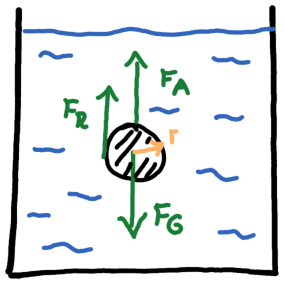
\includegraphics[width=5cm]{./bilder/StokesscheGleichung.png}
				\end{minipage}
				\newline
				\newline
				\newline
				\newline
				\begin{minipage}{12cm}
					\textbf{Laminare Rohrströmung (Gesetz von Hagen-Poiseuille)}
						\renewcommand{\arraystretch}{2.5}
						\begin{tabular}{ p{4cm} | p{7cm}}
							$V = \dfrac{\pi tR^4}{8 \eta l}\Delta p$	&	$V$ = geflossenes Fluidvolumen in $m^3$\\
							$\dfrac{dV}{dt} = \dfrac{\pi \overbrace{(p_1 - p_2)}^{\Delta p} R^4}{8 \eta l}$	& $R$ = Rohrradius in $m$\\
							$v(r) = -\dfrac{1}{4 \eta l} \cdot \Delta p \cdot (R^2-r^2)$ & $r$ = innerer Radius in Flüssigkeit in $m$\\
						\end{tabular}
						\renewcommand{\arraystretch}{1.5}
						\begin{tabular}{ p{4cm} | p{8cm} }
							& $\eta$ = dynamische Viskosität (Zähigkeit) in $Pa \cdot s$\\
							& $l$ = Länge des Rohres in $m$\\
							&	$\Delta p$ = Druckdifferenz zwischen Rohrenden in $Pa$\\
						\end{tabular} 
						\renewcommand{\arraystretch}{1}
				\end{minipage}
				\begin{minipage}{10cm}
					\vspace{-\ht\strutbox}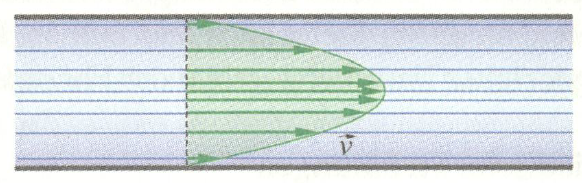
\includegraphics[width=6cm]{./bilder/Rohrstroemung1.png}
					\vspace{-\ht\strutbox}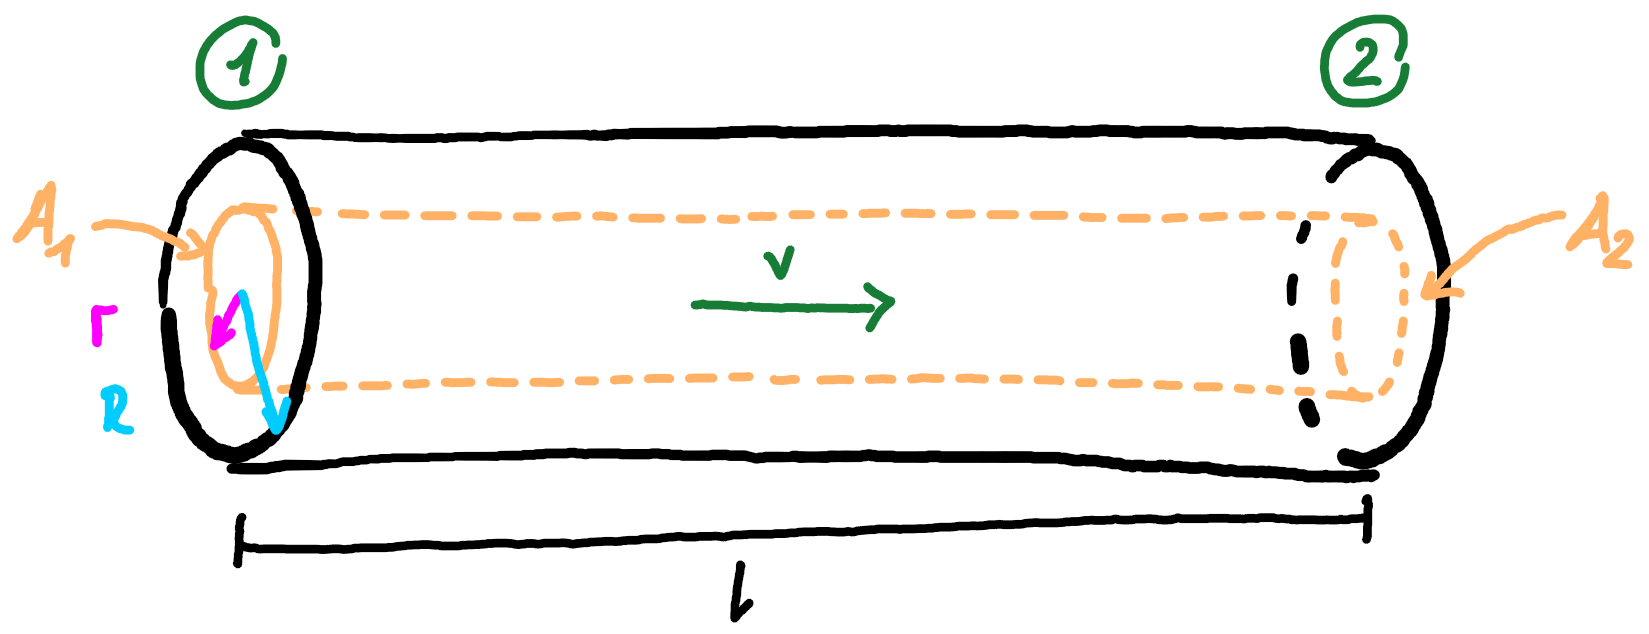
\includegraphics[width=6cm]{./bilder/Rohrstroemung2.png}
				\end{minipage}
				\newline
			\myparagraph{Turbulente Strömung}
			\newline
				\begin{minipage}{10.1cm}
					\textbf{Strömungswiderstand}
						\begin{flushleft}
						\end{flushleft}
						\renewcommand{\arraystretch}{2.5}
						\begin{tabular}{ p{3cm} | p{10cm}}
							$F_D = c_W A \dfrac{\rho v^2}{2}$	&	$F_D$ = Druckwiderstandskraft in $N$\\
							$F_W = c_W A_T \dfrac{\rho v^2}{2}$	&	$F_W$ = induzierte Widerstandskraft in $N$\\
							$F_A = c_A A_T \dfrac{\rho v^2}{2}$	&	$F_A$ = Auftriebskraft in $N$\\
							$c_W = \dfrac{F_W}{A}\dfrac{2}{\rho v^2}$	&	$c_W$ = Widerstandskoeffizient (Einheitslos)\\
						\end{tabular}
						\renewcommand{\arraystretch}{1.5}
						\begin{tabular}{ p{3cm} | p{10cm} }
							& $c_A$ = Auftriebskoeffizient (Einheitslos)\\
							& $\rho$ = Dichte Fluid in $\frac{kg}{m^3}$\\
							& $A$ = der Strömung entgegenstehender Körperquerschnitt in $m^2$\\
							& $A_T$ = zur Anströmrichtung parallele Ebene in $m^2$\\
							& $v$ = Strömungsgeschwindigkeit Fluid/Körper in $\frac{m}{s}$\\
						\end{tabular} 
						\renewcommand{\arraystretch}{1}
				\end{minipage}
				\begin{minipage}{10cm}
					\vspace{-\ht\strutbox}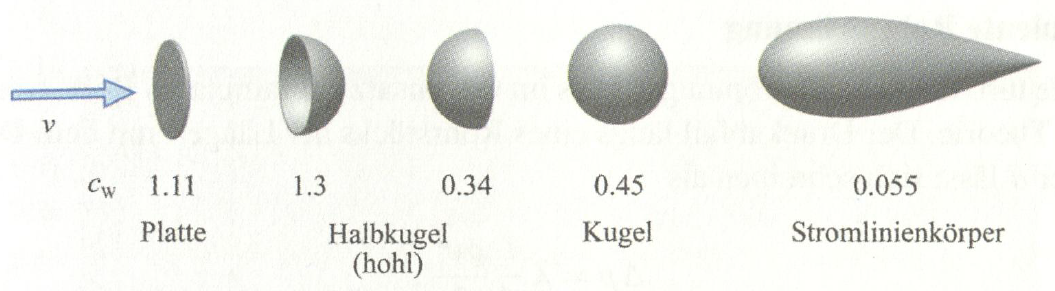
\includegraphics[width=9cm]{./bilder/WiderstandkoeffizientBeispiele.png}
				\end{minipage}
			
		\subsubsection{Dynamischer Auftrieb}
			\myparagraph{Magnus-Effekt}
				\newline
				Auftriebskraft, welche durch Rotation eines Körpers, welcher senkrecht von einer parallelen Strömung angeströmt wird, entsteht.
				\newline
				\newline
				\begin{minipage}[t]{13cm}
					\textbf{Zirkulation (für Zylinder)}
						\begin{flushleft}
							Mass für die Wirbelstärke in einer Strömung.
						\end{flushleft}
						\renewcommand{\arraystretch}{2.5}
						\begin{tabular}{ p{5cm} | p{7cm}}
							$\Gamma = \oint \vec{v} \cdot \mathrm{d} \vec{s} = 2 \pi r v_{Zyl} = 4 \pi^2 r^2 f$	&	$\Gamma$ = Zirkulation in $\frac{m^2}{s}$\\
						\end{tabular}
						\renewcommand{\arraystretch}{1.5}
						\begin{tabular}{ p{5cm} | p{7cm} }
							& $v$ = Anströmgeschwindigkeit Fluid in $\frac{m}{s}$\\
							& $v_{Zyl}$ = Umfangsgeschwindigkeit Zylinder in $\frac{m}{s}$\\
							& $f$ = Drehzahl Zylinder in $\frac{1}{s} = Hz$\\
						\end{tabular} 
						\renewcommand{\arraystretch}{1}
				\end{minipage}
				\begin{minipage}[t]{10cm}
					\vspace{-\ht\strutbox}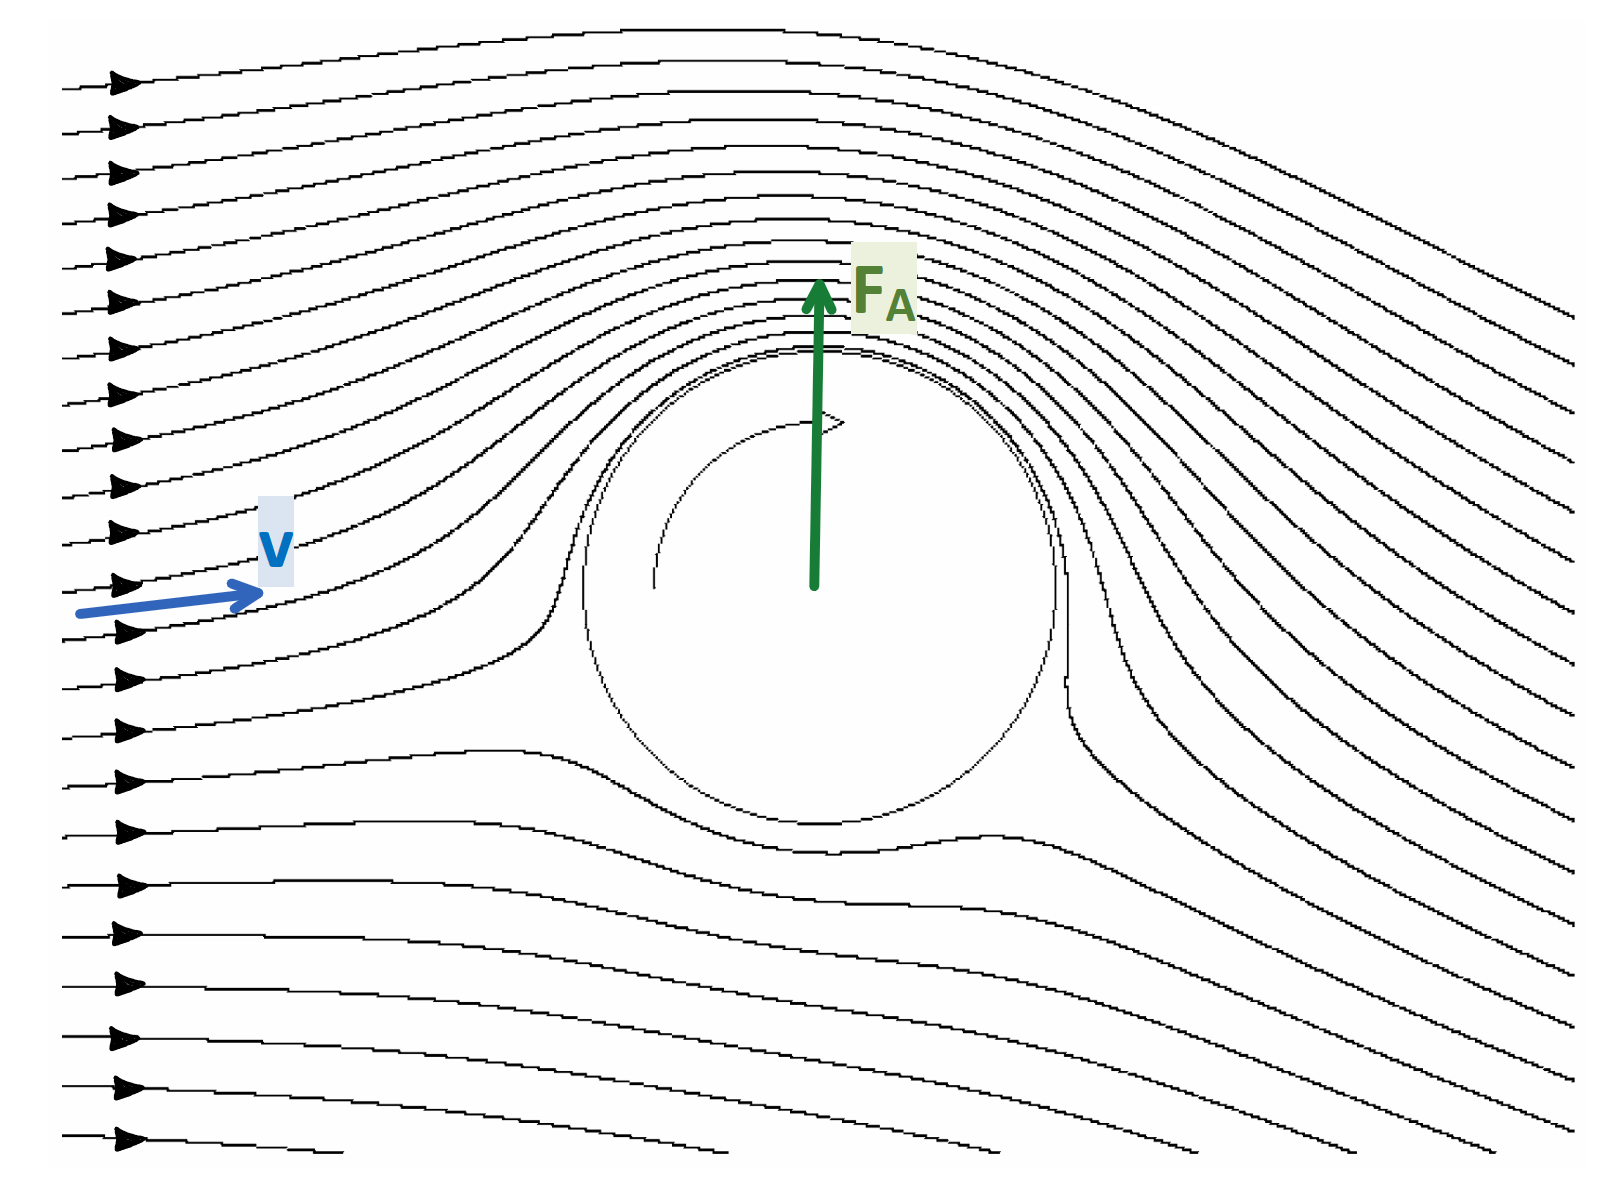
\includegraphics[width=6cm]{./bilder/MagnusEffekt.png}
				\end{minipage}
				\begin{minipage}[t]{13cm}
					\textbf{Kutta-Joukowski}
					\begin{flushleft}
						Proportionalität des dynamischen Auftriebs zur Zirkulation
					\end{flushleft}
					\renewcommand{\arraystretch}{2.5}
					\begin{tabular}{ p{5cm} | p{7cm}}
						$F_A = \rho lv \Gamma$	&	$F_A$ = Auftriebskraft in $N$\\
					\end{tabular}
					\renewcommand{\arraystretch}{1.5}
					\begin{tabular}{ p{5cm} | p{7cm} }
						& $\rho$ = Dichte Fluid in $\frac{kg}{m^3}$\\
						& $l$ = Länge Zylinder in $m$\\
						& $v$ = Anströmgeschwindigkeit Fluid in $\frac{m}{s}$\\
						& $\Gamma$ = Zirkulation in $\frac{m^2}{s}$
					\end{tabular} 
					\renewcommand{\arraystretch}{1}
				\end{minipage}
			
